% This is the chapter 'Modeling' to the "Hodgkin-Huxley neuron model V2.0 book"
% Last edited 2026.06.23

\iflatexml
\else
\minitoc
\fi


\ifx\magyar\undefined
\chapter[The V2.0 model]{The V2.0 model in a nutshell\label{sec:Modell-Nutshell}}
\else
\chapter[A V2.0 modell]{A V2.0 modell dióhéjban\label{sec:Modell-Nutshell}}
\fi

\quotationbox
{
"Everything should be made as simple as possible, but not simpler." Attributed to Albert Einstein.\\
}


The principle, suggested by A.~Einstein, means that while one should strip away unnecessary clutter, extra features, or overly complex jargon to achieve clarity, one must be careful not to remove so much that the core message or solution becomes meaningless or inaccurate.
For neurons (living matter), on the one side, it actually means that one should not reject quantities from the set of observed quantities
(the mass of the charge carrier and the pressure they cause) 
just because they are not present in a classical discipline (electricity) of the 
science, which once opon the time someone hypothesized (pre-decided?)
to describe neurons. Furthermore, one must include the proven new discoveries (effects and structures) made in the past eight decades (\gls{AIS}) and the
intentionally omitted
observations (heat emission and absorption; mechanical changes) which do not fit into the pre-authorized disciplinary theory.
On the other side, one must remove the foreign and fake ad hoc mechanisms and hypotheses (which contradict fundamental principles of science and elementary logics). 
All those issues were required to obscure that the current understanding does not match the experimental facts.

\else

\section[Modellezési elveink]{Modellezési elveink\label{sec:V2-0_ModelingPrinciples}}


A fenti, Albert Einsteintől származó, idézet azt jelenti,
hogy miközben eltávolítjuk a zavaró részleteket és 
az extra tulajdonságokat, vagy a megértés elősegítésére/nehezítésére használt komplikált
szakkifejezéseket, vigyáznunk kell arra, hogy ne hagyjunk el olyasmit,
aminek következtében az eredeti mondanivaló vagy a megoldás 
jelentését veszti vagy pontatlan lesz.
A neuronok (élő anyag) esetén ez azt jelenti, hogy nem hagyhatjuk el a
megfigyelt mennyiségek közül bármelyiket (a töltéshordozók tömegét és az általuk okozott nyomást), csupán azért, mert 
az nem szerepel abban a diszciplinában (elektromosságtan), amelyet az idők kezdetén valaki
a neuronok leírására alkalmasnak vélt (vagy előre elhatározott?).
Továbbá, figyelembe kell vennünk az utóbbi nyolc évtizedben  megalapozott új felfedezéseket (effektus vagy struktúra) (\gls{AIS}), 
és az eddigi előítéletes leírásokba nem illő és ezért szándékosan agyonhallgatott tényeket (hőtermelés és elnyelés, mechanikai változások).
Másrészt el kell távolítani az elméletből az idegen és
valótlan ad-hoc feltevéseket (amelyek ellentmondanak a tudomány
alapelveinek és az elemi logikának) (ellenirányban folyó azonos töltések árama, amelyek termelnek és elnyelnek hőt; energia felhasználás nélkül tömegeket mozgató rejtélyes protein erők; kommunikációs lehetőség nélkül kommunikáló szinkronizált ioncsatornák).
Ez utóbbiak azért kellettek, hogy elfedjék a tényt,
hogy jelen megértésünk nem felel meg a kísérleti tényeknek.
\fi

\ifx\magyar\undefined
\section[The abstract neuron]{The abstract neuron\label{sec:V2-0_AbstractNeuron}}

Nature uses an infinite variety of implementing neurons. 
In the \gls{CNS} 
they can cooperate
with each other, 'despite the extraordinary diversity and complexity of neuronal morphology and synaptic connectivity,
\textit{the nervous systems adopt \textbf{a number of
 basic principles}} for all neurons and synapses',
\cite{JohnstonWuNeurophysiology:1995}
independently from the infinitely complex molecular, biochemical and physiological details.
\index{Johnston Daniel}
\index{Wu Samuel Miao-sin }
We \textit{will base our holistic discussion on those general basic principles 
and create an 
\hyperlink{NeuronPhysical}
{'abstract physical neuron'}; a hypothetical element, which functions
essentially like a neuron},
skipping the 'implementation details' nature uses.
We essentially follow von Neumann's method in describing the foundations of
computing science~\cite{EDVACreport1945}: "we will base our considerations on a hypothetical element, which functions essentially like a neuron".
We need \hyperlink{Abstractions}
{different abstractions and approximations} 
(furthermore, \hyperlink{NonOrdinaryLaws}{'non-ordinary' laws} of science) for describing biological processes.
\index{ordinary laws}
However, an abstraction is usable
in practice only when paired with a generalization: the more abstract the assumption, the more general and widely applicable the concept or conclusion.
\textit{By abstractions, we can reduce the unbelievably detailed world into manageable pieces, and we can learn anything general.}
We must show which approximations are oversimplifications and which phenomena are misunderstood; measured, or interpreted in a wrong approach.


In our non-disciplinary science-based model (the 'abstract physical neuron', as we call it), a neuron (highly simplified) is an elastic sphere with two lipid layers (membrane) in an electrolyte, a similarly elastic insulating output tube (axon), and an incompressible, partially ionized electrolyte fluid with different compositions and concentrations inside and outside.
They contain ions, simple chemical molecules, and complex biological formations.
In the electolytes inside and outside  may have gradients and the ions move at continuously changing speeds that can vary by several orders of magnitude during operation. 
The lipid layer is partially permeable (controlled or uncontrolled) for the components above (channels, mainly ion channels).

\else

\section[Az absztrakt neuron]{Az absztrakt neuron\label{sec:AbstractNeuron}}

A természet végtelenül változatos módokon valósít meg neuronokat.
A központi idegrendszerben (\gls{CNS}) ezek egymással együtt tudnak működni, mivel 'despite the extraordinary diversity and complexity of neuronal morphology and synaptic connectivity,
\textit{the nervous systems adopt \textbf{a number of
 basic principles}} for all neurons and synapses',
\cite{JohnstonWuNeurophysiology:1995}
azok rendkívül összetett molekuláris, biokémiai és fiziológiai 
részleteik ellenére.
\index{Johnston Daniel}
\index{Wu Samuel Miao-sin}
Átfogó tárgyalásunkban ezekre az általános elvekre támaszkodunk
és egy \hyperlink{NeuronPhysical}
{'abstract physical neuron'}-nak nevezett hipotetikus elemet
hozunk létre, ami lényegében úgy működik, mint egy neuron;
átugorva az "implementációs részleteket".
Lényegében Neumann Jánosnak a számítástudomány alapelveit 
leíró munkájában~\cite{EDVACreport1945} vezetett be:
"we will base our considerations on a hypothetical element, which functions essentially like a neuron".

Különböző  \hyperlink{Abstractions}
{absztrakciók és közelítések},
(továbbá, \hyperlink{NonOrdinaryLaws}{a tudomány 'rendetlen' (non-ordinary) törvényeinek} ) felhasználásával  írjuk le a biológiai
folyamatokat.
\index{rendetlen törvények}
Azonban a gyakorlatban egy absztrakció csak akkor használható,
ha egy általánosítással párosítjuk. Minél absztraktabb egy feltevés,
annál szélesebb körben használható a fogalom vagy következtetés.
\textit{Az absztrakciók által a hihetetlenül gazdag világot
kezelhető darabokra bontjuk és általános dolgokat tanul\-hatunk.}
Meg kell mutatnunk hogy melyik közelítés túlegyszerűsítés
és milyen tapasztalaokat értettünk félre; mértünk vagy értelemeztünk rosszul.

A nem diszciplináris, tudományos alapú modellünkben, a neuron (erős egyszerűsítésekkel),
egy olyan rugalmas gömb, amit két lipid réteg (membrán) határol, 
és egy hasonlóképpen rugalmas szigetelő csőben (axon) végződik.
Ez a gömb összenyomhatatlan, részben ionizált elektrolitot tartalmaz,
és a membrán külső és belső oldalán az elektrolitok 
koncentrációja és kémiai összetétele nagyon eltérő.
Az oldatban vannak ionok, egyszerű molekulák és összetett biológiai képződmények.
Ezekben az elektrolitokban, kívül és belül, gradiensek létezhetnek
és az ionok folyamatosan, akár nagyságrendekkel, változó sebességekkel mozoghatnak a működés során. 
A lipid réteg részben (ellenőrzött módon vagy szabadon)  átjárható
(csatornákon, főleg ion csatornákon keresztül) a fenti komponensek számára.
\fi




\begin{figure}
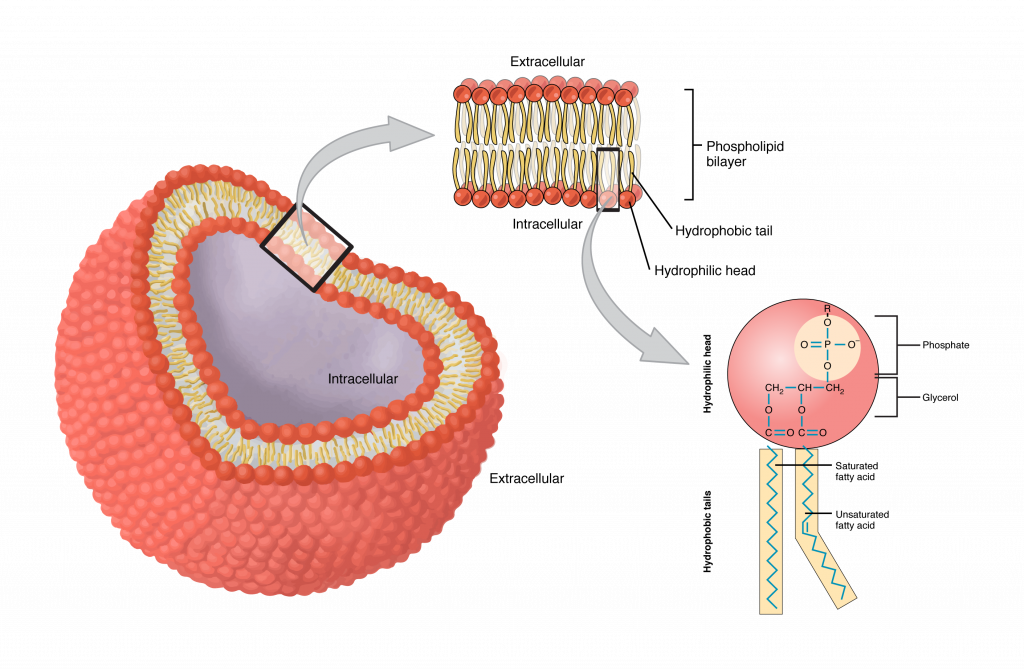
\includegraphics[width=.65\textwidth]{fig/phospholipid1.png}
\caption{\label{fig:LipidSphere}
\href{https://open.oregonstate.education/aandp/chapter/3-1-the-cell-membrane}{A simulated picture of the neuron membrane}.
We can consider the membrane as a closed surface (in our idealist view, a sphere), being slightly opened at an attached tube, the axon. For certain processes, we can also consider just a tiny section as a planar piece, see also Figure~\ref{fig:MembraneComposition}
}	
\end{figure}
 



\begin{figure}
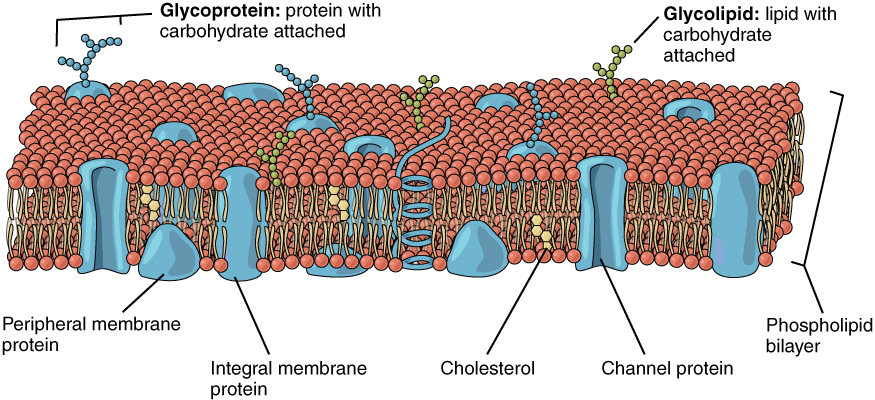
\includegraphics[width=.65\textwidth]{fig/Lipid_Bilayer_With_Various_Components.jpg}
\caption{\label{fig:MembraneComposition}
The cell membrane is a phospholipid bilayer containing many different molecular components, including proteins and cholesterol, some with carbohydrate groups attached.
Lipids are amphiphilic molecules that like water on one side and repel water
on the other side due to the hydrocarbon chains. In contact to
water lipids spontaneously form double layers (see Figure \ref{fig:MembraneComposition}) that are the basic building blocks of biomembranes.
}	
\end{figure}

\ifx\magyar\undefined
\section[The abstract ion channels]{The abstract ion channels \label{sec:AbstractIon channels}}

Embedded in the wall of the membrane, a smaller amount of (controlled 
and uncontrolled) ion channels are scattered.
Between the membrane and the axon, there is an array of a large amount of uncontrolled ion channels (the Axon Initial Segment \gls{AIS}). 
The elastic wall of the membrane is covered with ion layers, and therefore, a potential difference is created there (the resting potential).
The membrane represents \textit{a confined space in which ions behave differently from in an infinite space}; furthermore, it significantly alters the properties of the few-nanometer-thick electrolyte layer near the membrane. In this layer, the concentration and potential change significantly with the distance from the membrane due to interactions between the membrane's ion layers and the electrolyte.
Ion packages (spikes) sent by other neurons can enter the internal volume through controlled inputs (synapse).

\else

\section[Az absztrakt ioncsatornák]{Az absztrakt ioncsatornák \label{sec:AbstractIon channels}}
A membrán falába ágyazva, nagyobb számú vezérelt és kisebb számú vezérlés nélküli ioncsatorna, a membrán és az axon között
pedig egy nagyon sok vezérletlen ioncsatornát tartalmazó ion tömb 
(az Axon Initial Segment \gls{AIS}) helyezkedik el.
A rugalmas membrán falát ionrétegek borítják, és ezért
potenciál különbség ("nyugalmi potenciál") keletkezik rajta.
\textit{A membrán olyan zárt teret képez, amelyben az ionok a szabad térben
ismerttől eltérő módon viselkednek}; továbbá, a membránon levő feszültség jelentősen megváltoztatja az elektrolitok tulajdonságait a 
membránhoz közel eső néhány nanométer vastagságú rétegben. 
Ebben a rétegben a koncentráció és a potenciál jelentősen függ
a membrántól való távolságtól; ami a membrán ionrétegei és az
elektrolit közötti kölcsönhatás következménye.
A más neuronok által küldött ion csomagok (spikes) a belső térfogatba
vezérelt bemeneteken (szinapszisokon)  át léphetnek be.
\fi


%The membrane functions as a \hyperlink{ControlTheory}{\gls{PID} control circuit}.
\ifx\magyar\undefined
\section[Neuron's states]{Neuron's states \labellabel{sec:Model-NeuronStates}}
Under a small external influence, a neuron remains in its resting state and regulates itself through non-controlled ion channels in its membrane.
If the external influence exceeds a threshold, the controlled channels in the wall suddenly release a large amount of ions into the internal space, putting the neuron into a transient state.
The membrane potential changes suddenly (within a few dozen nanoseconds), and, due to the mutual repulsion of ions, the pressure acting on the membrane wall and the ion concentration in the layer near the membrane also increase significantly and suddenly. At this point, the disciplines of electricity and thermodynamics can be combined: the pressure and the electric field are proportional to the number of ions in the volume.
The forces exerted on ions, calculated in a disciplinary way, are falsified 
in the sense that the other discipline also contributes inseparably; in a strict sense, neither of the two disciplines alone can describe ions' motion.
The detailed analysis shows that the elastic energy during the action potential
is about two orders of magnitude higher than the electrical energy, but the 
amount of ions is about three oders of magnitude lower than that of the non-dissociated molecules.
It that situation, the two effects are of the same order of magnitude,
so that they can modulate each other. The electric charge on the membrane's wall 
would produce a simple discharge current. However, its charge carriers are
delivered by the damped oscillation of the electrolyte (a soliton) generated by the membrane.
The amplitude of the soliton changes the number of the charge carriers delivered,
so physiology measures an oscillating discharge current (that generates
a potential wave known as \gls{AP}). No significant mass transfer
takes place.

\else

\section[A neuron állapotai]{A neuron állapotai\label{sec:Model-NeuronStates}}
Kis külső behatás esetén, a neuron nyugalmi állapotában marad és szabályozza állapotát a falban levő vezérletlen ioncsatornákon át.
Ha a külső behatás túllép egy küszöbértéket, a falban levő vezérelt 
ioncsatornákon át nagy mennyiségű ion kerül a belső térbe,
és a neuron tranziens állapotba kerül.
A membrán potenciál értéke hirtelen (néhány tucat nanosecundum alatt)
megváltozik, és, az ionok kölcsönön taszítása miatt, megnő a
membrán falra ható nyomás; továbbá, az ionok egyidejűleg megnövelik 
a membrán-közeli rétegekben a koncentrációt.
Ezen a ponton lehet kombinálni az elektromosságtan és a termodinamika
diszciplináit: a nyomás és az elektromos tér egyránt a térfogatrészben
található ionok számával arányos.
Az ionokra ható, diszciplináris módon számított erők olyan értelemben
nem valódiak, hogy a másik diszciplina következtében elválaszthatatlanul fellépő erők összeadódnak; szigorúan véve, egyik diszciplina sem tudja
leírni az ion mozgását: az általa ismert erő alapján az ion mozgásának nem olyannak kell lenni. 
A részletes analízis azt mutatja, hogy az \gls{AP} során a
rugalmas energia körülbelül két nagyságrenddel nagyobb,
mint az elektromos energia; viszont az ionok száma kb. három nagyságrenddel kisebb, mint a nem disszociált molekuláké.
%The detailed analysis shows that the elastic energy during the action potential
%is about two orders of magnitude higher than the electrical energy, but the 
%amount of ions is about three oders of magnitude lower than that of the non-dissociated molecules.
Ebben a helyzetben a két hatás ugyanabba a nagyságrendbe esik,
így modulálni tudják egymást.
Az elektromos kisülés egy egyszerű kisülési áramot jelentene.
Azonban, az elektrolitnak a membrán által generált rezgőmozgása (a soliton) szállítja a töltéshordozókat.
A soliton amplitúdója változtatja a szállított töltéshordozók számát,
így a fiziológiai elektromos mérés egy oszcilláló kisülési áramot
érzékel (ami az \gls{AP} néven ismert potenciálhullámot generálja).
A jelenség során nincs jelentős tömeg átvitel.
\fi

\ifx\magyar\undefined
\section[The non-disciplinary behavior]{The non-disciplinary behavior\label{sec:Model-Non-disciplinary}}
Since \textit{the same physical action generates the voltage gradient and the concentration gradient} (and, consequently, the pressure), they are inseparable and proportional to each other.
Generating a voltage change (clamping, direct current, magnetic pulse) or a pressure change (ultrasound, mechanical, shock waves) on the membrane mutually cause the other to change. Inputting ions (synaptic input) generates both changes.
The control circuit tries to restore the resting state, during which the mentioned changes decrease proportionally.
The transient state of the neuron can, in principle, be described by any of the mentioned quantities, but, as a practical matter, \textit{the effects of changes in the other entities must also be taken into account}: \textit{no single discipline, alone, can describe the changes}.
The elastic membrane implements an almost critically damped vibration, but the "vibrating mass" and the "spring force" are constantly changing.
In an electric resonant circuit, the capacitor's voltage and capacitance change due to the finite amount of charge.
\textit{The pressure wave caused by a force shock and the voltage wave caused by a voltage shock describe the same effect}.
In both cases, the other effect must be taken into account to some extent: an infinitesimal movement of the ion also changes both the pressure and the voltage.
Changes in pressure and charge alter the membrane's thickness (and therefore its capacity), and both voltage and pressure can cause a structural change (phase change, "melting") in the lipid chains that make up the membrane.
\else

\section[A nem-diszciplináris viselkedés]{A nem-disciplináris viselkedés\label{sec:Model-Non-disciplinary}}
Mivel \textit{a feszültség és a koncentráció gradienst is ugyanaz a
fizikai hatás generálja}, a két gradiens egymással arányos és
egymástól elválaszthatatlan.
Feszültség változás (clamping, közvetlen áram bevezetés, mágneses impulzus) vagy nyomás változás (ultrahang, mechanikai, lökéshullám)
a membránon a másik változást is előidézi.
Ionok belépése (szinaptikus bemenet) is mindkét változást előidézi.
A neuron vezérlőegysége megpróbálja helyreállítani a nyugalmi állapotot,
aminek során az említett változások arányosan csökkennek.
A neuron tranziens állapota, elvben, a két említett menníiség mindegyikével leírható. Praktrikus szempontból azonban 
\textit{a másik változó értékében bekövetkezett változás hatása is számításba
veendő: egyetlen diszciplina, egyedül, nem tudja leírni a változásokat}.
A rugalmas membrán egy csaknem kritikusan csillapított rezgést valósít meg; de a "regő tömeg" és a "rugóerő" folyamatosan változik.
Egy elektromos rezgőkörben a kondenzátor feszültsége és kapacitása a
töltés véges mennyisége miatt változik.
\textit{Az erőlökés miatti nyomáshullám és a feszültséglökés miatti
feszültséghullám ugyanazt a fizikai hatást írják le.}
Mindkét esetben figyelembe kell venni valamilyen mértékben a másik 
hatást is: az ion egy kis mozgása egyszerre változtatja 
a nyomást és a feszültséget is.
A nyomás és a töltés változása a membrán vastagságát (és ezért kapacitását) is változtatja, továbbá a feszültség és a nyomás is 
okozhat strukturális változást (phase change, "melting")
a membránt alkotó lipid láncokban.
\fi
\index{melting!lipids}


\ifx\magyar\undefined
Here, the difference comes to light: the carrier of the \gls{EM} interaction has no mass, while the thermodynamic one does.
In the case of the pressure wave, the speed is naturally finite (mass must be moved). For the electric wave, there are laws regarding only instantaneous interaction; so, they must be adapted to \textit{slow ion current}s based on physical assumptions.
\index{slow current}
It is simpler to describe the generation of the action potential as an electrical oscillation, and its propagation as a pressure wave (although this only represents the wave front well:
the \gls{AP} lasts as long as there is a non-equilibrium charge in the neuron: the repulsion between the excess ions pushes the ions out of the closed space, so the intensity of the wave continuously decreases).
Hyperpolarization is described in the electrical view as a capacitive current in the sequential oscillator circuit, in the thermodynamic view as a suction effect occurring in the opposite phase of the membrane. 
In both cases, however, it must be taken into account that charge and mass are inseparable in ions, and that their cross-disciplinary effects significantly reduce the applicability of the disciplinary laws.
Furthermore, as our force analysis suggests, the ions' motion results 
an interference between the longitudinal thermodynamic oscillation of elastic origin
and a discharge process of electrical origin. 

\else
Itt jön napvilágra az a lényegi különbség, hogy az \gls{EM}
sugárzás hordozójának nincs nyugalmi tömege, míg a termodinamikai kölcsönhatás hordozójának van.
A nyomáshullám esetén a sebesség magától értetődően véges
(tömeget kell mozgatni).
Elektromos hullám esetén, csak az azonnali kölcsönhatásra vonatkozó
törvények vannak; azokat (fizikai megfontolások alapján) 
adaptálni kell lassú áramok esetére.\index{lassú áram}
Az \gls{AP} keltését elektromos rezgőkörként, továbbítását pedig
nyomáshullámként egyszerűbb leírni.
Az \gls{AP} mindaddig tart, amíg nem-egyensúlyi töltés van a
neuronban: a többlet ionok közötti taszítás kitolja az ionokat a
zárt térfogatból, így az intenzitás folyamatosan csökken.
A hiperpolarizációt az elektromos szemléletben a szekvenciális rezgőkör
kapacitív áramaként írhatjuk le, a termodinamikai szemléletben pedig 
a membrán ellentétes rezgési fázisában fellépő szívóhatásként. 
Mindkét esetben számításba kell vennünk, hogy az ionok töltése és tömege 
elválaszthatalanok, és azok diszciplinákon átívelő hatása 
jelentősen csökkenti a diszciplináris törvények alkalmazhatóságát.
Amint azt erő-analízisünk mutatja, az ionok mozgása a rugalmas eredetű
termodinamikus oszcilláció és az elektromos eredetű kisülési folyamat
eredőjeként áll elő.
\fi
 
\ifx\magyar\undefined
\section[The neuron as Carnot-engine]{The neuron as Carnot-engine\label{sec:Model-CarnotEngine}}
In simple words, a neuron combines different disciplines; it works like a two-tact biological internal combustion engine, and can be described theoretically as a special Carnot-type thermodynamic engine, see section~\ref{sec:Physics-Thermodynamics}. The synaptic input currents operate the ignition. The influx of $Na^+$ ions acts like an explosion, producing a large pressure impulse due to electrical repulsion between ions; see section~\ref{sec:Physics-Speculations}. The neuron's volume remains practically unchanged (representing an iso-volume process), and the pressure wave vibrates the particles (including dissociated ions) as a longitudinal wave, and the resulting offset potential moves the ions out of the neuron through the only available output channel: the axon. The pressure wave is similar to a sound wave, with negligible material transport. 
The force analysis shows that the pressure wave
causes a longitudinal vibration, while the changed potential adds
a potential-dependent longitudinal force component for moving the ions.

\else

\section[A neuron mint Carnot-gép]{A neuron mint Carnot-gép\label{sec:Model-CarnotEngine}}
Egyszerűen fogalmazva, a neuron két diszciplinát kombinál össze.
Úgy működik, mint egy két-ütemű biológiai belső égésű motor,
és elméletileg egy speciális Carnot-féle termodinamikai gépnek
tekinthető.
A szinaptikus bemenő áram gyújtásként hat. A $Na^+$ ionok rendkívül gyors beáramlása robbanásként hat,
és nagy nyomás- és feszültség-gradienst hoz létre.
A neuron térfogata gyakorlatilag változatlan marad (azonos térfogatú folyamat),
és a nyomáshullám rezgeti a részecskéket (köztük a disszociált ionokat) longitudinális hullámként,
a keletkezett többlet potenciál pedig mozgatja az ionokat az egyetlen lehetséges  kilépési útvonal: az axon felé. 
A nyomáshullám egy hanghullámhoz hasonló, elhanyagolható anyagszállítással.
Az erők analízise azt mutatja, hogy a nyomáshullám longitudinális rengést okoz, a megváltozott potenciál pedig egy longitudinális 
erőkomponenssel járul hozzá az ion mozgatásához.
\fi

\ifx\magyar\undefined
The two-tact engine, in the first stroke, the pressure impulse invests energy into compressing the elastic membrane and starting a compression wave (a soliton). In the first tact, the elastic membrane pumps out some electrolyte, and in the second tact it pumps in part of the electrolyte (the driving force is a combined thermoelectrical/mechanical force rather than some magic battery). The pumping goes through the ion channels in the \gls{AIS}, which "resists" it, thereby generating a potential wave known as \gls{AP}; well described by electricity. The force analysis shows that the pressure wave
causes a longitudinal vibration, while the changed potential adds
a potential-dependent longitudinal force component for moving the ions. Compressing the electrolyte
produces heat, as evidenced by a rise in temperature. The expansion consumes heat, as evidenced by a decrease in temperature. These are well-understood processes in thermodynamics.
However, they are still unexplained in biophysics, although they were observed
seven decades ago~\cite{HeatProductionNeuron:1958}.
The elastic membrane functions as a damped oscillator, which, in its negative amplitude phase, reverses the direction of electrolyte flow (and, consequently, the direction of the current carried by the ions).
In the discipline of electricity (when using the serial $RC$ model), it can be interpreted as a capacitive current, which in physiology is observed as hyperpolarization that inverts the polarity of the output voltage.
The ions represent both mass and charge simultaneously, and, correspondingly, one can observe, in addition to the electrical potential wave, mechanical, optical, and other features changing.
In different disciplines, pressure and voltage represent the same phenomenon, using concepts from various disciplines.
Both waves propagate with the speed of the carrier.

\else

A kétütemű motor működésének első ütemében a nyomás erőlökése
energiát fordít a  rugalmas membrán összenyomásába és elindít 
egy nyomáshullámot (soliton).
Az első ütemben a rugalmas membrán elektrolitot pumpál ki
az \gls{AIS} ioncsatornáin keresztül, a második ütemben pedig részben visszaszívja azt. A csatornák "ellenállnak",
ezért az \gls{AP} néven ismert potenciálhullámot hozzák létre;
a jelenséget az elektromosságtan jól leírja. 
(a hajtóerő tehát egy kombinált termodinamikai/elektromos erő,
és nem valamiféle állandó vagy mágikusan változó  feszültségű
feszültséggenerátor)
A folyadék összenyomása hőt termel, ami hőmérséklet emelkedésben 
nyilvánul meg.
A kiterjedés hőt fogyaszt, ami hőmérséklet csökkenésben nyilvánul meg.
A termodinamikában ezek jól ismert folyamatok, 
de a biofizika annak ellenére nem tudja magyarázni, hogy a folyamatokat
már hét évtizeddel ezelőtt megfigyelték.~\cite{HeatProductionNeuron:1958}.
A rugalmas membrán egy csillapított oszcillátorként működik,
ami, a negatív amplitúdójú fázisban, megfordítja az elektrolite folyadék
áramlásának irányát (beleértve a szállított ionok áramlásának irányát is).
Ez a jelenség az elektromosságtanban (amikor soros  $RC$  modellt használjuk), kapacitív áramként értelmezhető, amit a fiziológia 
hiperpolarizációként figyel meg, ami megfordítja a kimenő feszültség polaritását.
Az ionok egyidejűleg jelentenek tömeget és töltést,
és ennek megfelelően, az elektromos potenciál hullám mellett,
mechanikai, optikai és egyéb tulajdonságok is változnak. 
A különböző diszciplinákban a nyomás és a feszültség 
ugyanazt a jelenséget mutatják a megfelelő diszciplina saját
fogalmai szerint, amitz az is alátámaszt, hogy mindkét hullám a hordozó sebességével terjed.
\fi

\ifx\magyar\undefined
\section[Physics of neuron]{Physics of neuron\label{sec:Model-Physics}}

\else
\section[A neuron fizikája]{A neuron fizikája\label{sec:Model-Physics}}
Az ionok kölcsönhatásakor mindig kétféle térrel kell dolgoznunk: a determinisztikus 'azonnali' elektromos térből
és egy sztochasztikus lassú erőtérből származó elsődleges erőkkel,
amelyek nagyságrendeket változhatnak
nanométeres távolságokon, továbbá függenek az ionok kémiai természetétől és a biológiai struktúrák változatos 
irányú és nagyságú ellenerőket is kiválthatnak. 
Mindezek figyelembe vételéhez nagyon részletes numerikus 
szimulációk vagy nagyon jó közelítések szükségesek.
Megközelítésünk olyan tér- és időbeli szakaszokra 
oszt\-ja fel a biológiai történéseket, amelyekben --jó közelítéssel-- egy domináns és egy korrigáló kölcsönhatás lép fel.
\fi

 
\ifx\magyar\undefined
Today, two major branches of disciplinary theories compete
for being applied to describe the neuronal operation \cite{CriticalElectricity:2018,ThermodynamicAPDrukarch:2022,PerspectivesNerveSignalPropagation:2024,ComparisonHHandSoliton:2010,HH_Potential_Controversies_2017,PiezoelectricNeuron:2025}. Those cited references also compare those theories.
The 2-decade-old Heimburg-Jackson thermodynamic theory is trying to break in alongside or displace the 7-decade-old all-electric Hodgkin-Huxley theory. The two theories apply one of the scientific disciplines developed for inanimate nature, unchanged, to living nature. There are unexplained observations for each of the two theories, and neither can describe the biological neuron's functioning without contradictions. 
In a disciplinary view, there is no chance of the two theories fusing. Although they can describe a wider range of phenomena together, the conditions under which they are applicable exclude their joint use. Moreover, to conceal contradictions and fill gaps, biophysics assumes (typically unspecified protein) mechanisms that contradict the fundamental principles of physics, and some of them even the disciplinary laws.

\else

Manapság két fő diszciplináris elmélet verseng,
hogy a neuronális működés leírására használják~\cite{CriticalElectricity:2018,ThermodynamicAPDrukarch:2022, PerspectivesNerveSignalPropagation:2024, ComparisonHHandSoliton:2010, HH_Potential_Controversies_2017, PiezoelectricNeuron:2025}.
Az idézet közlemények össze is hasonlítják az elméleteket.
A két évtizedes Heimburg-Jackson termodinamikus elmélet
próbál betörni a hét évtizededes Hodgkin-Huxley elmélet mellé,
vagy akár helyettesíteni azt.
Mindkét elmélet egy, az élettelen természetre kifejlesztett diszciplinát alkalmaz, változatlan formában, az élő természetre. 
Mindkét elméletben vannak megmagyarázatlan megfigyelések,
és egyik sem tudja ellentmondásmentesen leírni a biológiai 
neuron funkcionalitását.
A diszciplináris szemlélet alapján nincs esély a két elmélet fúziójára.
Bár együtt a jelenségek egy szélesebb körét tudják leírni,
alkalmazhatóságuk feltételei kizárják együttes használatukat.
Továbbá, az ellentmondások feloldására és a magyarázatlan 
jelenségek kiküszöbölésére, a biofizika olyan,
(jellemzően meghatározatlan protein), mechanizmusokat 
tételez fel, amelyek ellentmondanak a fizika alapelveinek és
néhányuk még a disciplináris törvényeknek is.
\fi

\ifx\magyar\undefined
The electrical view essentially stems from the (Nobel Prize-winning) work of Hodgkin and Huxley \cite{HodgkinHuxley:1952}. They could not make a perfect job, mainly due to the lack of
discoveries made several decades later, including ours, about handling
the finite speed of the biological ionic currents (and, due to that, the dynamic features), which drastically change
their conclusions. In contrast with their \textit{empirical description}, which delivered mathematically formulated measured observations, our discussion, although it follows essentially
the same principles, reinterprets and pinpoints the used fundamental terms, sets up a physical model, and \textit{explains} the physically underpinned processes. ``However, the theory could not explain the physical
phenomena such as reversible heat changes, density changes,
and geometrical changes observed in the experiments'' \cite{ComparisonHHandSoliton:2010}.
The thermodynamic view roots in the (possibly Nobel-prize-winning)
idea of Heimburg and Jackson \cite{SolitonPropagation:2005}. They proposed that the action potential is essentially a sound wave (a soliton). "However, there are several other questions that this has to answer like ion flow involvement in nerve signal propagation as stated by the \gls{HH} model and also the faster propagation in myelinated nerves than in unmyelinated" \cite{ComparisonHHandSoliton:2010}.
If we consider that the ion flow means charge propagation in a membrane tube where the specific capacity depends on the thickness (of the myelin sheath) of the wall \cite{VeghUnifiedCrossdisciplinaryModel:2026}, the faster propagation is not mysterious anymore.
Those apparent contradictions are simply consequences of ions' non-disciplinary features.
By using the correct (non-disciplinary) discussion of the phenomena,
we can explain all those observations in more detail in section~\ref{sec:Physics-Unified}.
Given that
our model natively connects charge and mass of ions~\cite{VeghNon-ordinaryLaws:2025}, it has a good chance of explaining the missing phenomena.

\else

Az elektromos szemlélet lényegében Hodgkin and Huxley (Nobel-díjas) \cite{HodgkinHuxley:1952} munkájából ered.
Nem végezhettek tökéletes munkát, főleg a csak évtizedekkel később
ismertté vált felfedezések hiánya miatt. Az utóbbiak között van
a mi felfedezésünk, a véges sebességű biológiai áramok kezeléséről (és ennek következtében a dinamikus viselkedésről), ami drasztikusan
megváltoztatja következtetéseiket.
Matematikailag megfogalmazott mérési eredményeken alapuló tapasztalati leírásukkal ellentétesen, a mi tárgyalásunk, bár lényegében ugyanazon alpelveket követi, újra értelmezi és pontosítja 
az alapfogalmakat, valóban fizikai modellt ad, és \textit{megmagyarázza} a fizikailag alátámasztott folyama\-tokat.
"However, the theory could not explain the physical
phenomena such as reversible heat changes, density changes,
and geometrical changes observed in the experiments"\cite{ComparisonHHandSoliton:2010}.
A termodinamikus szemlélet Heimburg and Jackson \cite{SolitonPropagation:2005} (esetleg Nobel-díjas) ötletén alapszik.
Javaslatuk szerint az akciós potenciál lényegében hanghullám (soliton).
"However, there are several other questions that this has to answer like ion flow involvement in nerve signal propagation as stated by the \gls{HH} model and also the faster propagation in myelinated nerves than in unmyelinated" \cite{ComparisonHHandSoliton:2010}.
Ha azt tekintjük, hogy az ion folyam egy membrán csőben terjedő 
töltést jelent, ahol a specifikus kapacitás a(z esetleg myelinréteggel borított) fal vastagságától függ~ \cite{VeghUnifiedCrossdisciplinaryModel:2026}, már a gyorsabb terjedés sem misztikus.
A bemutatott ellentmondások egyszerűen az ionok nem-diszciplináris tulajdonságainak következményei.
A tapasztalatok helyes (nem-diszciplináris) tárgyalásával
a tapasztalatok teljes körűen magyarázhatók.
Mivel modellünk természetes módon összekapcsolja a töltést és a tömeget~\cite{VeghNon-ordinaryLaws:2025}, jó esélye van a még hiányzó tapasztalatok magyarázására is.
\fi



The excellent textbook's statement that "the resting membrane potential results
from the separation of charge across the
cell membrane"~\cite{PrinciplesNeuralScience:2013} is only half the truth; we tell the second half in section~\ref{sec:Physics-MembraneElectricity}. 
We refute their statement that "%by discussing how 
resting ion channels
establish and maintain the resting potential"~\cite{PrinciplesNeuralScience:2013}, page 126.
The ion channels are passive players. The interplay of 
the lipid condenser and the electrolytes on both sides
of the permeable membrane establishes the resting potential, and ionic gradients maintain it.
The textbook separates the neuron membrane's states into resting and transient states. 
It introduces resting and transient ion channels,
but does not introduce that the different physical processes in those states need different models. 
As we show in section~\ref{sec:Physics-Unified}, \textit{two different physical mechanisms
operate in the resting and the transient states}, so two different models are needed for describing the same components.

A primary reason neurophysiology has been misguided is that it has in mind a static picture of the dynamic life of neurons.
It started from the static
inanimate anatomic microscopic pictures, continued
with the static clamping investigations (where
the negative feedback of an external electric circuit eliminates the natural gradients) and underpinning the
theory by analyzing frozen (inanimate) samples
by electron microscopes.
Those investigations revealed a tremendous amount of crucial details,
but they obscured the idea
that those samples are just snapshots of a permanently
changing system.
Neuroscience projected the mechanisms of the static resting state to the dynamic transient state and attempted
to understand the transient state 
as perturbations~\cite{PerturbationNeuralComputation:2002} to the  (entirely different) resting state.
Of course, that attempt required more and more ad hoc non-scientific assumptions.
We agree that "Understanding and predicting molecular responses
in single cells upon chemical, genetic or mechanical perturbations is a core question in biology."~\cite{PerturbationSingleCell:2023}
However, it is not possible without understanding that the transient state is a state on its own right,
with different physical mechanisms, rather than a perturbation of the entirely different resting state.

Due to the lack of the needed expertize in physics,
biophysics introduced the idea of the "whatnot"~\cite{Schrodinger:1992} protein mechanisms.
Claims such as "pumps [by using protein mechanisms] \dots transport ions \textit{against their
electrical and chemical gradients}"~\cite{PrinciplesNeuralScience:2013}, page 101, 
or "the flux of ions through ion channels is passive,
requiring \textit{no expenditure of metabolic energy} by the
channels."~\cite{PrinciplesNeuralScience:2013}, page 107, are as scientific as in the pre-Newtonian age,
there was a notion related to Aristotelian philosophy. This concept gave credence to the “theory” that the celestial spheres and, later on, the planets were pushed or moved by celestial movers, celestial intelligences, or angels against physical forces. Life science does not have its laws of motion, in the sense as Newton's Laws in physics, at least at cellular level. 
\index{law of motion}

The book~\cite{PrinciplesNeuralScience:2013} asks the central questions, "How do ionic [i.e., electrical and chemical] gradients contribute to the resting membrane potential? What prevents
the ionic gradients from dissipating by diffusion of
ions across the membrane through the resting channels?"
However, it leaves them essentially open by giving only a qualitative answer, discussing only membrane permeability, without explaining how the resting potential is created.
%
We demonstrate in section~\ref{sec:Physics-MembraneElectricity} that classical methods of electricity enable us to calculate the membrane's potential resulting from charge separation and polarization, why and how its resting value is created, furthermore, how it is regulated.
We make some physically plausible assumptions to provide numerical figures.

Our results underpin that "the crucial system in biology isn't a molecule or a molecular class whatsoever, but the interface created by biomolecules in water"~\cite{LivingSystemPhysics:2021}. We add that mainly
physical processes at various speeds (instead of molecular classes such as proteins) and ionic gradients (instead of protein mechanisms) control the processes.
More precisely, inseparable thermodynamic and electrical processes set up and maintain the potential established by the electrical and thermodynamic backbone defined by the lipid/protein structure of the cell and the ionic solutions it contains. It is one of the frequent cases when 
one effect implements a functionality (the backbone closely defines the frames of the operation), and the other (in this case, combined thermodynamics and electricity) corrects it when it implements a complex operational (dynamical) functionality:
"stimulated phase transitions enable the phase-dependent processes to replace each other ... one process to build and the other
to correct"~\cite{BiologicalConservationLaw:2017}.

\ifx\magyar\undefined

\section[Differences to V1.0]
{Essential differences to the V1.0 model\label{sec:Modell-Differences}}

\else

\section[Eltérések a V1.0-tól]
{Eltérések a V1.0 modelltől\label{sec:Modell-Differences}}

\fi


\ifx\magyar\undefined

\else

\fi